%%%%%%%%%%%%%%%%%%%%%%%%%%%%%%%%%%%%%%%%%%%%%%%%%%%%%%%%%%%%%%%%%%%%%%%%%%%%%%%
%%%%%%%%%%%%%%%%%%%%%%%%%%%%%%%%%%%%%%%%%%%%%%%%%%%%%%%%%%%%%%%%%%%%%%%%%%%%%%%
\chapter{Разработка модуля абстрактной интерпретации для системы статического
анализа Borealis}
\label{chapter:implementation}
%%%%%%%%%%%%%%%%%%%%%%%%%%%%%%%%%%%%%%%%%%%%%%%%%%%%%%%%%%%%%%%%%%%%%%%%%%%%%%%
%%%%%%%%%%%%%%%%%%%%%%%%%%%%%%%%%%%%%%%%%%%%%%%%%%%%%%%%%%%%%%%%%%%%%%%%%%%%%%%
В данном разделе описываются основные этапы разработки модуля абстрактной 
интерпретации для системы статического анализа Borealis, который реализует
описанную ранее технологию. Рассматривается архитектура прототипа и его
основные компоненты.

%%%%%%%%%%%%%%%%%%%%%%%%%%%%%%%%%%%%%%%%%%%%%%%%%%%%%%%%%%%%%%%%%%%%%%%%%%%%%%%
\section{Архитектура прототипа}
%%%%%%%%%%%%%%%%%%%%%%%%%%%%%%%%%%%%%%%%%%%%%%%%%%%%%%%%%%%%%%%%%%%%%%%%%%%%%%%
Под прототипом понимается программный модуль, реализующий предложенную методику
объединения абстрактной интерпретации и метода ограниченной проверки моделей.
Высокоуровневая схема работы прототипа приведена на 
рисунке~\ref{image:NewBorealisOverview}. Структура модулей разрабатываемого
прототипа приведена ниже~(рисунок~\ref{image:prototypeArchitecture}).
\begin{figure}[h!]
\center{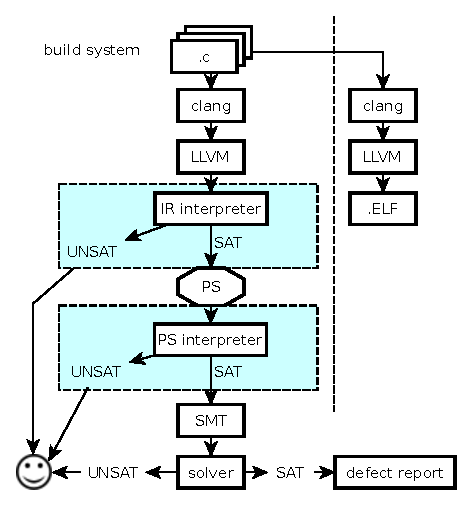
\includegraphics[width=0.8\linewidth]{NewBorealisOverview}}
\caption{Архитектура разрабатываемого прототипа}
\label{image:NewBorealisOverview}
\end{figure}
\begin{figure}[h!]
\center{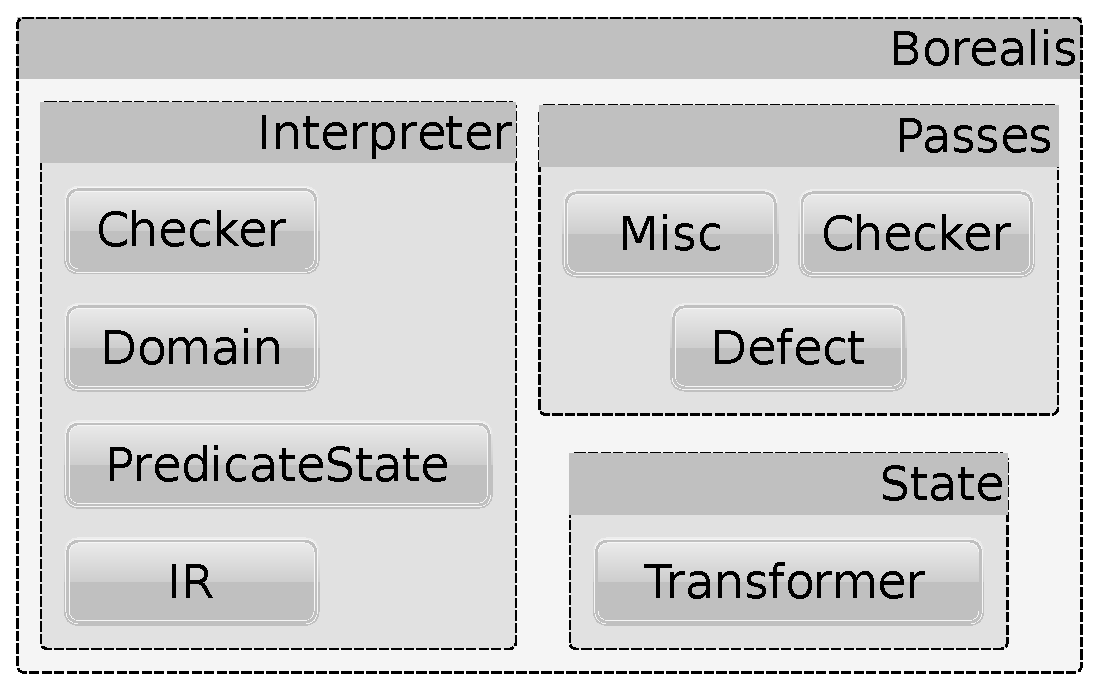
\includegraphics[width=0.8\linewidth]{prototypeArchitecture}}
\caption{Структура модулей разрабатываемого прототипа}
\label{image:prototypeArchitecture}
\end{figure}

Данный модуль основывается на предложенной ранее технологии и содержит 
реализации следующих функций: абстрактная интерпретация модуля LLVM, 
абстрактная интерпретация PS, поиск ошибок по результатам интерпретации. 
При этом прототип может быть сконфигурирован для запуска в режиме интерпретации
только LLVM, только PS или и LLVM, и PS. Рассмотрим более подробно все 
компоненты разрабатываемого модуля.

%%%%%%%%%%%%%%%%%%%%%%%%%%%%%%%%%%%%%%%%%%%%%%%%%%%%%%%%%%%%%%%%%%%%%%%%%%%%%%%
\section{Разработка модуля для системы Borealis}
%%%%%%%%%%%%%%%%%%%%%%%%%%%%%%%%%%%%%%%%%%%%%%%%%%%%%%%%%%%%%%%%%%%%%%%%%%%%%%%
В разработку модуля абстрактной интерпретации для системы Borealis входит 
написание новых классов для анализа кода, а также расширение функциональности 
уже существующих классов. В ходе работы были изменены некоторые компоненты 
системы и было реализовано несколько новых компонентов~(рисунок
~\ref{image:prototypeArchitecture}). Компонент \texttt{Interpreter}
содержит реализацию всех классов, связанных с абстрактной интерпретацией:
абстрактных доменов, состояний, интерпретаторов и  т.д. Компонент \texttt{Passes}
содержит проходы LLVM, которые выполняют анализ и модификацию исходного кода.
Компонент \texttt{State} содержит описание и реализацию PS.

%%%%%%%%%%%%%%%%%%%%%%%%%%%%%%%%%%%%%%%%%%%%%%%%%%%%%%%%%%%%%%%%%%%%%%%%%%%%%%%
\subsection{Компонент \texttt{Interpreter}}
%%%%%%%%%%%%%%%%%%%%%%%%%%%%%%%%%%%%%%%%%%%%%%%%%%%%%%%%%%%%%%%%%%%%%%%%%%%%%%%
Компонент \texttt{Interpreter} содержит реализации всех классов, необходимых для
проведения абстрактной интерпретации. В нем содержится два класса: 
\texttt{Interpreter} и \texttt{OneForOneInterpreter}. 

\texttt{Interpreter} --- класс, который выполняет абстрактную интерпретацию 
модуля LLVM~(рисунок~\ref{image:irInterpretation}). Он наследуется от класса
\texttt{llvm::InstVisitor}, который реализует шаблон проектирования 
Visitor~\cite{visitor} для инструкций LLVM. Исходный код класса 
\texttt{Interpreter} приведен в приложении.

Класс \texttt{OneForOneInterpreter} содержит реализацию метода
\texttt{bool check(PredicateState::Ptr state, PredicateState::Ptr query, const 
DefectInfo\& di)}, который выполняет интерпретацию PS \texttt{state} и 
проверяет, выполняется ли на нем свойство \texttt{query}.

Также, в компоненте \texttt{Interpreter} содержатся следующие пакеты:
\begin{itemize}
\item \texttt{Checker} --- данный пакет содержит реализацию классов, которые 
выполняют поиск ошибок по результатам интерпретации модуля LLVM. Он содержит 
следующие классы:
    \begin{itemize}
    \item \texttt{NullDereferenceChecker} --- класс, для поиска ошибок 
    некорректного разыменовывания указателей~(рисунок~\ref{image:ndChecker});
    \item \texttt{OutOfBoundsChecker} --- класс, для поиска ошибок выхода за 
    границы массива~(рисунок~\ref{image:oobChecker});
    \item \texttt{OutOfBoundsVisitor} --- вспомогательный класс, который 
    выполняет рекурсивный обход абстрактных доменов для поиска выхода за границы
    массива.
    \end{itemize}
\item \texttt{Domain} --- данный пакет содержит реализации абстрактных доменов для системы типов LLVM~(см. подраздел~\ref{section:domains}). В нем содержатся 
следующие классы:
    \begin{itemize}
    \item \texttt{Domain} --- абстрактный класс абстрактного домена, от которого
    наследуются все абстрактные домены;
    \item \texttt{AggregateDomain} --- реализация агрегатного домена;
    \item \texttt{IntegerIntervalDomain} --- реализация интервального домена для 
    целых чисел;
    \item \texttt{FloatIntervalDomain} --- реализация интервального домена для 
    чисел с плавающей точкой;
    \item \texttt{FunctionDomain} --- реализация домена функций;
    \item \texttt{PointerDomain} --- реализация домена указателей;
    \item \texttt{IntervalWidening} --- реализация операторов widening для 
    интервальных доменов;
    \item \texttt{DomainFactory} --- данный класс реализует шаблон 
    проектирования фабрика~\cite{factory} для абстрактных доменов. Также в нем 
    есть методы для разбора константных выражений 
    LLVM~(\texttt{llvm::ConstantExpr}).
    \end{itemize}

    Также в пакете \texttt{Domain} содержатся вспомогательные классы с 
    реализацией решетки целых чисел с фиксированной разрядностью.

\item \texttt{IR} --- в данном пакете содержатся реализации различных 
вспомогательных классов, используемых при интерпретации LLVM IR:
    \begin{itemize}
    \item \texttt{State} --- реализация состояния программы для LLVM IR. Для 
    оптимизации использования памяти, было решено хранить в состоянии 
    программы только информацию о локальных переменных. Глобальные переменные 
    было решено хранить в единственном экземпляре для всего модуля. Данный 
    класс хранит в себе хеш-таблицу, которая каждой локальной переменной 
    функции ставит в соответствие абстрактный домен, который ее описывает. Так 
    как состояния программы приходится достаточно часто копировать, было решено 
    вместо обычной хеш-таблицы использовать хеш-таблицу, которая копируется 
    только при записи~(copy-on-write map);
    \item \texttt{BasicBlock} --- класс-обертка над базовым блоком LLVM
    \texttt{llvm::BasicBlock}, который хранит состояние программы до
    выполнения соответствующего блока и после;
    \item \texttt{Function} --- класс-обертка над функцией LLVM
    \texttt{llvm::Function}, который хранит состояние программы до 
    выполнения функции и после. Также в нем хранится отображение базовых блоков
    LLVM объекты типа \texttt{BasicBlock};
    \item \texttt{Module} --- класс-обертка над модулем LLVM
    \texttt{llvm::Module}, который хранит информацию о функциях 
    программы;
    \item \texttt{GlobalVariableManager} --- класс, отвечающий за работу с 
    глобальными переменными. Он выполняет топологическую сортировку графа
    глобальных переменных~(глобальные переменные в LLVM могут зависеть друг от
    друга, но при этом они объявлены в модуле без учета всех зависимостей);
    \item \texttt{ConditionSplitter} --- вспомогательный класс, который 
    выполняет <<разделение>> абстрактных доменов при условных переходах.
    \end{itemize}
\item \texttt{PredicateState} --- в данном пакете содержатся реализации 
различных вспомогательных классов, используемых при интерпретации PS. Он 
содержит в себе два класса:
    \begin{itemize}
    \item \texttt{State} --- состояние программы для PS;
    \item \texttt{ConditionSplitter} --- вспомогательный класс, который 
    выполняет <<разделение>> абстрактных доменов при условных переходах в 
    Choice PS.
    \end{itemize}
\end{itemize}

В компоненте \texttt{Interpreter} также содержатся реализации различных 
вспомогательных функций~(операторы сравнения и функции печати для классов LLVM
и т.д.) в файлах \texttt{Util.hpp} и \texttt{Util.cpp}.

%%%%%%%%%%%%%%%%%%%%%%%%%%%%%%%%%%%%%%%%%%%%%%%%%%%%%%%%%%%%%%%%%%%%%%%%%%%%%%%
\subsection{Компонент \texttt{State/Transformer}}
%%%%%%%%%%%%%%%%%%%%%%%%%%%%%%%%%%%%%%%%%%%%%%%%%%%%%%%%%%%%%%%%%%%%%%%%%%%%%%%
Анализ и преобразование PS выполняется с помощью трансформеров (Transformer). 
Механизм трансформеров, используемый в системе Borealis, реализует шаблон 
CRTP~(Curiously Recurring Template Pattern)~\cite{crtp} и шаблон 
Visitor~\cite{visitor}. Трансформеры являются удобным инструментом для анализа 
и трансформации PS. Они позволяют обходить как весь PS, так и его части.

\texttt{PropertyPredicateFilterer} выполняет фильтрацию предикатов в 
анализируемом PS: он удаляет из PS предикаты, которые работают с property~(это
некоторые дополнительные свойства объектов, которые используются в Borealis и
не имеют значения для интерпретации).

\texttt{Interpreter} --- трансформер, который проводит абстрактную интерпретацию
PS. Он обходит все термы и предикаты в полученном PS и на доменах,
соответствующих используемым в выражении переменным, вызывает абстрактные 
операторы, соответствующие анализируемому выражению.

\texttt{QueryChecker} --- трансформер, который выполняет проверку выполнения
какого-либо свойства программы по результатам интерпретации~(то есть по 
состоянию программы на выходе PS).

%%%%%%%%%%%%%%%%%%%%%%%%%%%%%%%%%%%%%%%%%%%%%%%%%%%%%%%%%%%%%%%%%%%%%%%%%%%%%%%
\subsection{Компонент \texttt{Passes/Transformer}}
%%%%%%%%%%%%%%%%%%%%%%%%%%%%%%%%%%%%%%%%%%%%%%%%%%%%%%%%%%%%%%%%%%%%%%%%%%%%%%%
Как упоминалось ранее, в компоненте \texttt{Passes} содержатся проходы LLVM,
которые выполняют анализ и преобразование исходного кода программы. В пакет
\texttt{Passes/Misc} был добавлен новый проход
\texttt{IRInterpreterPass}, который выполняет интерпретацию модуля, поиск 
ошибок в модуле и сохранение информации о найденных ошибках в класс 
\texttt{DefectManager}. \texttt{IRInterpreterPass} --- это \texttt{ModulePass}, 
то есть он запускается один раз для каждого модуля программы.

В пакете \texttt{Passes/Defect} были внесены изменения в класс 
\texttt{DefectManager}. \texttt{DefectManager} --- это \texttt{ModulePass}, 
который хранит информацию о всех проверяемых ошибках. В него было добавлено
новое поле, которое хранит информацию об ошибках, которые гарантированно не 
выполняются в программе~(эта информация получается по результатам AI).

В пакете \texttt{Passes/Checker} были внесены изменения в шаблонный класс
\texttt{CheckHelper}. Метод \texttt{check} был изменен так, что вызов SMT 
решателя осуществляется только если в \texttt{DefectManager} нет информации
о проверяемой ошибке после проведения абстрактной интерпретации.

%%%%%%%%%%%%%%%%%%%%%%%%%%%%%%%%%%%%%%%%%%%%%%%%%%%%%%%%%%%%%%%%%%%%%%%%%%%%%%%
\section{Резюме}
%%%%%%%%%%%%%%%%%%%%%%%%%%%%%%%%%%%%%%%%%%%%%%%%%%%%%%%%%%%%%%%%%%%%%%%%%%%%%%%
В данном разделе была рассмотрена реализация прототипа описанной ранее 
технологии объединения абстрактной интерпретации и метода ограниченной проверки 
моделей на основе системы Borealis. Показана архитектура разработанного 
прототипа и описаны основные модули.